\documentclass[12pt]{article}
\usepackage[letterpaper,margin={1.5cm}]{geometry}
\usepackage{amsmath, amssymb, amsfonts}
\usepackage[utf8]{inputenc}
\usepackage[T1]{fontenc}
\usepackage[spanish]{babel}
\usepackage{tikz}
\usepackage{graphicx,enumitem}
\usepackage{multicol}
\setlength{\marginparsep}{12pt} \setlength{\marginparwidth}{0pt} \setlength{\headsep}{.8cm} \setlength{\headheight}{15pt} \setlength{\labelwidth}{0mm} \setlength{\parindent}{0mm} \renewcommand{\baselinestretch}{1.15} \setlength{\fboxsep}{5pt} \setlength{\parskip}{3mm} \setlength{\arraycolsep}{2pt}
\renewcommand{\sin}{\operatorname{sen}}
\newcommand{\N}{\ensuremath{\mathbb{N}}}
\newcommand{\Z}{\ensuremath{\mathbb{Z}}}
\newcommand{\Q}{\ensuremath{\mathbb{Q}}}
\newcommand{\R}{\ensuremath{\mathbb{R}}}
\newcommand{\C}{\ensuremath{\mathbb{C}}}
\newcommand{\I}{\ensuremath{\mathbb{I}}}
\graphicspath{{../imagenes/}{imagenes/}{..}}
\allowdisplaybreaks{}
\raggedbottom{}
\setlength{\topskip}{0pt plus 2pt}
\newcommand{\profesor}{Edward Y. Villegas}
\newcommand{\asignatura}{M\'ETODOS NUM\'ERICOS}
\newcommand{\diff}[3]{\frac{d^{#3} #1}{d#2^{#3}}}
\newcommand{\pdiff}[3]{\frac{\partial^{#3} #1}{\partial#2^{#3}}}
\newcommand{\abs}[1]{\left| #1 \right|}
\begin{document}
  \pagestyle{empty}
  \begin{minipage}{\linewidth}
    \centering
    \begin{tikzpicture}[very thick,font=\small]
      \node at (2,6) {
\includegraphics[width=3.5cm]{logoudem}};
      \node at (9.5,6) {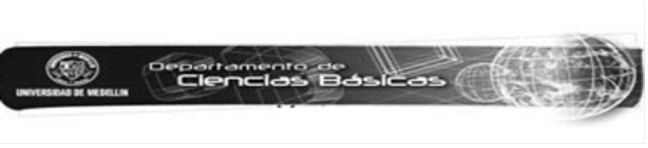
\includegraphics[width=9cm]{cbudem}};
      \node[fill=white,draw=white,inner sep=1mm] at (9.5,5.05) {\bf Permanencia con calidad, Acompa\~nar para exigir};
      \node[fill=white,draw=white,inner sep=1mm] at (7.5,4.2) {\Large\bf DEPARTAMENTO DE CIENCIAS B\'ASICAS};
      \draw (0,0) rectangle (18,3.5);
      \draw (0,2.5)--(18,2.5) (0,1.5)--(18,1.5) (15,4.2)--(18,4.2) node[below,pos=.5] {CALIFICACI\'ON} (15,2.5)--(15,7)--(18,7)--(18,3.5) (8.4,0)--(8.4,1.5) (15,0)--(15,1.5) (10,1.5)--(10,2.5);
      \node[right] at (0,3.2) {\bf Alumno:}; \node[right] at (15,3.2) {\bf Carn\'e:};
      \node[right] at (0,2.2) {\bf Asignatura:};
      \node at (6,1.95) {\asignatura};
      \node[right] at (10,2.2) {\bf Profesor:};
      \node at (15,1.95) {\profesor};
      \node[right] at (0,1.2) {\bf Examen:};
      \draw (3.8,.9) rectangle (4.4,1.3); \node[left] at (3.8,1.1) {Parcial:};
      \draw (3.8,.2) rectangle (4.4,.6); \node[left] at (3.8,.4) {Previa:};
      \draw (7.4,.9) rectangle (8,1.3); \node[left] at (7.4,1.1) {Final:};
      \draw (7.4,.2) rectangle (8,.6); \node[left] at (7.4,.4) {Habilitaci\'on:};
       \node at (4,1.1) {X}; % Parcial
      \node[right] at (10,.5) {3 - 8 - 9}; % Número de grupo
      \node[right] at (10,1.) {17 Marzo de 2016}; % Fecha de presentación
      \node[right] at (8.4,1.05) {\bf Fecha:}; \node[right] at (8.4,.45) {\bf Grupo:};
      \node[align=center,text width=3cm,font=\footnotesize] at (16.5,.75) {\centering\bf Use solo tinta\\y escriba claro};
    \end{tikzpicture}
  \end{minipage}
Presente el examen en el \textbf{grupo matriculado}, de lo contrario será anulado.
Para el desarrollo de los cálculos puede usar \textbf{exclusivamente calculadora} (no se permite el uso de portátil o celulares en el examen), y al final del examen, encontrará una \textbf{hoja de formulas} para su ayuda.
Todo valor reportado debe aproximarse a \textbf{5 CIFRAS SIGNIFICATIVAS} con \textbf{REDONDEO SIMÉTRICO} (no es necesario en enteros). Recuerde el uso del separador decimal acorde a la \textbf{NTC}.
Indique \textbf{clara y explícitamente la respuesta final} de cada pregunta en \textbf{lapicero} (requisito en caso de reclamación), y \textbf{justifique todas sus respuestas y procedimientos. Si algún elemento solicitado, en teoría no puede realizarse, indíquelo y justifique por que no se puede realizar lo solicitado. Si necesita espacio adicional, use el respaldo de las hojas para el procedimiento (no se permiten hojas extras)}.
\textbf{Nota: Solo los valores dados en los enunciados se permitirá un uso diferente a las 5 cifras significativas.}
\vspace{-.5cm}
  \begin{enumerate}[leftmargin=*,widest=9]
     \item (\(1.2\)) Una caída en \textit{bungee jumping} puede modelarse su aceleración como:
\begin{equation*}
a = g + \frac{\frac{1}{2}\mu v^2}{\mu (L-y) + 2L}
\end{equation*}
donde \(\mu=5.44\) es la relación de masas de la cadena y el cuerpo lanzado, la longitud de la cadena es \(L = 4.15m\) y la aceleración debida a la gravedad para Medellín es \(g=9.78m/s^2\). Si la velocidad alcanzada en el punto de sensación de ingravidez (\(a=0m/s^2\)) era de \(v=17m/s\), ¿cual debía ser la distancia recorrida en caída \(y\) medida en metros? Aproxime usando \(y=1m\) con un método abierto a 3 iteraciones.

\textbf{R/} Primero, se reemplazarán los valores constantes y unidades en la expresión por comodidad de manipulación, y simplificamos.
\begin{eqnarray}
0 m/s^2 & = & \left( 9.78 + \frac{\frac{1}{2}5.44 (17)^2}{5.44 (4.15-y) + 2(4.15)} \right) m/s^2 \nonumber \\
0 & = & 9.78 + \frac{786.08}{- 5.4400 y + 30.876} \label{ec_bungee}
\end{eqnarray}
El lado derecho de la ecuación \ref{ec_bungee} es la función a la que deseamos buscar la raíz, cuya indicación de condición inicial es \(y_0=1m\).
Para este punto puede seleccionar cualquier método abierto (formulas al final del parcial): Newton, Secante, Secante modificada y M\"uller.
Para ilustrar, se usará el método de Newton.
\begin{eqnarray}
\diff{f(y)}{y}{} & = & \diff{ \left(9.78 + \frac{786.08}{- 5.4400 y + 30.876} \right) }{y}{} \nonumber \\
f^{\prime}(y) & = & \frac{4276.3}{\left(- 5.4400 y + 30.876\right)^{2}} \label{ec_bungee_dif}
\end{eqnarray}
Reemplazando ec.\ref{ec_bungee_dif} y ec.\ref{ec_bungee} en la formula de Newton, se obtiene la forma recursiva ec.\ref{ec_newton}, donde se observa que para la condición inicial se satisfacen condiciones mínimas para la aplicación del método (existencia de la función y sus primeras dos derivadas, así como primera derivada distinto de cero). Por este motivo, se procede a usar el método, pero aún no se asegura convergencia (es necesario revisar la evolución del error absoluto).
\begin{equation}
y_{i+1} = y_i - \frac{\left(9.78 + \frac{786.08}{- 5.4400 y + 30.876} \right)}{\left( \frac{4276.3}{\left(- 5.4400 y + 30.876\right)^{2}} \right)} \label{ec_newton}
\end{equation}
Finalmente aplicando la formula de Newton para el caso especifico obtenemos
\begin{equation*}
\begin{array}{|c|c|c|c|}
\hline
n & x_i & g(x_i) & \epsilon_{ay} \\
\hline
1 & 1 & -5.1554 & 6.1554 \\
2 & -5.1554 & -23.926 & 18.771\\
3 & -23.926 & -112.83 & 88.904\\
\hline
\end{array}
\end{equation*}
Se obtiene como respuesta a tres iteraciones \(y = -112.83\). Se observa que cada iteración produce un valor más distante que el anterior (el error absoluto aumenta), por lo cual el resultado encontrado no sirve como aproximación (el método diverge).
Tambien puede basarse en el criterio del teorema de punto fijo, teniendo en cuenta que \[ g(y) = y - \frac{f(y)}{f^{\prime}(y)}. \]
    \item Dado el polinomio de tercer grado \(P_3(x) = 2x^3 + 3x - 1 + 4x^2\)
    \begin{enumerate}[label=\alph*]
    \item (\(0.4\)) ¿Cual es la diferencia del total de operaciones realizadas para evaluar \(P_3(x)\) entre la forma tradicional y el algoritmo de Horner?

\textbf{R/} Sabemos que el número de sumas es igual tanto en la forma tradicional como en Horner (número de sumas es \(n-1\)), de forma que esta cantidad no aporta a la diferencia. Respecto a las multiplicaciones, la forma tradicional realiza más multiplicaciones que la forma de Horner, y su diferencia es
   \[ \frac{n(n+1)}{2} - n = \frac{n(n-1)}{2},\]
   en la cual reemplazando \(n= 3\), la diferencia será \(3\).
    \item (\(1.0\)) Evalué usando el algoritmo de Horner \(P_3(3)\) y \(P^\prime_3(3)\). \textbf{Recordar:} La evaluación de la derivada debe construirse con el propio algoritmo de Horner y no derivando directamente.

\textbf{R/} Evaluamos \(P_3(3)\), que ordenado es \(P_3(x) = 2x^3+4x^2+3x-1\).
\begin{eqnarray*}
b_3& = & 2\\
b_2 &= & 2\cdot 3 + 4 = 10\\
b_1 &= & 10 \cdot 3 + 3 = 33\\
b_0 &= & 33 \cdot 3 - 1 = 98 = P_3(3)
\end{eqnarray*}
Ahora se evaluá la derivada con ayuda del polinomio \(Q\) formado por los coeficientes residuales de Horner (distintos de \(b_0\)), \(Q(x) = 2x^2 + 10x +33\).
\begin{eqnarray*}
b_2 &= & 2\\
b_1 & = & 2\cdot 3 + 10 = 16\\
b_0 &= & 16 \cdot 3 + 33 = 81 = P_3^{\prime}(3)
\end{eqnarray*}
   \item (\(0.4\)) Realice la primera iteración del método de Newton-Horner con valor inicial \(x_0=3\) para \(P_3(x)\).

\textbf{R/} Para aplicar la primera iteración de Newton-Horner al polinomio \(P_3(x)\) con \(x_0 = 3\), sustituimos los valores antes encontrados en la formula (disponible al final del examen).
  \begin{equation*}
  x_1 = 3 - \frac{98}{81} = 1.7901
  \end{equation*}
   \end{enumerate}
   \item Dado el siguiente conjunto de datos.
   \begin{equation*}
   \begin{array}{|c|c|c|}
   \hline
   x_i & f(x_i) & f^\prime(x_i) \\
   \hline
   0 & -1 & 2\\
   2 & 0 & -1\\
   3 & 2 & 0\\
   \hline
   \end{array}
   \end{equation*}
   \begin{enumerate}[label=\alph*]
   \item (\(0.4\)) Con el conjunto de datos dado, justifique que método de interpolación debe aplicar.

\textbf{R/} Dado que se indica información de la derivada ademas de la evaluación directa, corresponde el método de interpolación de Hermite.
   \item (\(1.2\)) Acorde al método de interpolación que indico, realice la interpolación del conjunto de datos. \textbf{Desarrollo:} Indique cada paso de procedimiento (polinomios y tablas auxiliaras, y polinomio interpolante).

\textbf{R/} Se construye para la interpolación de Hermite la tabla auxiliar de diferencias divididas, en la variable \(z\) (transformación de \(x\) en la cual se duplican sus valores al tener información de la evaluación de la función y de la derivada de la misma).
\begin{equation*}
\begin{array}{|c|c|c|c|c|c|c|}
\hline
z_i & f_i & f_{i, i+1} & f_{i, i+1, i+2} & f_{i, i+1, i+2, i+3}& f_{i, i+1, i+2, i+3, i+4} & f_{i, i+1, i+2, i+3, i+4}\\
\hline
0 & -1 & 2       & -0.75000 & 0       & 0.41667 & -0.83332\\
0 & -1 & 0.50000 & -0.75000 & 1.2500  & -2.0833 &\\
2 & 0  & -1      & 3   & -5 &&\\
2 & 0  & 2  & -2  &&&\\
3 & 2  & 0       &&&&\\
3 & 2  &&&&&\\
\hline
\end{array}
\end{equation*}
Ahora, usando los primeros elementos de las diferencias divididas construimos el polinomio interpolante de Hermite
\[H_5(x) =-1 + 2x -0.75000x^2 + 0.41667x^2(x-2)^2-0.83332 x^2(x-2)^2(x-3). \]
\item (\(0.4\)) Aproxime el valor correspondiente a la función para \(x=3.001\).

\textbf{R/} Sabemos del teorema de la aproximación polinomial que para poder acotar el error de la aproximación, el valor de interes debe estar contenido en el intervalo de la interpolación, que para este caso es \(0 \leq x \leq 3\). Como \(x=3.001\) esta por fuera, no se puede usar el polinomio interpolante.
   \end{enumerate}
  \end{enumerate}
\begin{center}
\textbf{Hoja de fórmulas}
\end{center}
{\large
\[
\begin{array}{cc}
x_{i+1} = g(x_i) \qquad & \qquad |g^\prime(x_i)| < 1 \\
x_{i+1} = x_i - \frac{f(x_i)}{f^\prime(x_i)} \qquad & \qquad x_{i+1} = x_i - \frac{P(x_i)}{Q(x_i)} \\
x_{i+1} = x_i - \frac{f(x_i) \Delta x}{f(x_i + \Delta x) - f(x_i)} \qquad & \qquad x_{i+2} = x_{i+1} - \frac{f(x_{i+1}) (x_{i+1}-x_i)}{f(x_{i+1}) - f(x_i)} \\
b_n = a_n \qquad & \qquad
b_k = b_{k+1}x_0 + a_k \\
L_{n, i}(x) = \prod\limits_{\substack{j=0\\ i \neq j}}^n \frac{x - x_j}{x_i - x_j} \qquad & \qquad
P_n(x) = \sum\limits_{i = 0}^n f(x_i)L_{n,i}(x) \\
f\left[x_i, x_{i+1}\right] = \frac{f(x_{i+1})-f(x_i)}{x_{i+1}-x_i} \qquad & \qquad
f\left[ x_i, x_{i+1}, \ldots, x_{j-1}, x_j\right] = \frac{f\left[x_{i+1}, \ldots, x_{j-1}, x_j\right] - f\left[ x_i, x_{i+1}, \ldots, x_{j-1} \right]}{x_j - x_i} \\
z_{2i} = z_{2i+1} = x_i \qquad & \qquad
H_{2n+1} = f(x_0) + \sum\limits_{k=1}^{2n+1} f\left[x_0, \ldots, x_k\right] \prod\limits_{i = 0}^{k-1}(x-x_i) % \\
\end{array}
\]
}
\end{document}
